% Common preamble for PIGMIE patent figures (A4).
% Drawing conventions:
%   - A4 portrait
%   - Sans-serif throughout (Helvetica)
%   - "Fig. N" sentence-case caption near top
%   - Page "N/total" at top centre
%   - Reference numerals outside boxes via leader lines
%   - ALL CAPS labels in component boxes
%   - Reactor uses north-east-lines hatched fill
%   - Scene uses double-line border
%   - Module enclosures use dashed line with internal numeral

\documentclass[a4paper,10pt]{article}
\usepackage[top=2.5cm,bottom=1.0cm,left=2.5cm,right=1.5cm]{geometry}
\usepackage[T1]{fontenc}
\usepackage{helvet}
\renewcommand{\familydefault}{\sfdefault}
\usepackage{amsmath,amssymb,bm}
\usepackage{tikz}
\usetikzlibrary{shapes,shapes.geometric,shapes.misc,arrows.meta,positioning,fit,calc,backgrounds,decorations.pathreplacing,decorations.markings,patterns}
\pagestyle{empty}
\setlength{\parindent}{0pt}

\tikzset{
  % Component box: ALL CAPS label inside, no numeral inside
  cbox/.style={draw, rectangle, minimum height=1.0cm, minimum width=2.4cm,
               align=center, line width=0.5pt, font=\small},
  cbox-tall/.style={cbox, minimum height=1.6cm},
  cbox-wide/.style={cbox, minimum width=3.0cm},
  cbox-narrow/.style={cbox, minimum width=1.8cm, font=\footnotesize},
  % Reactor / physical medium: hatched fill
  reactor/.style={cbox, pattern=north east lines, pattern color=black!70},
  % Scene: double-line border
  scenebox/.style={cbox, double, double distance=1.2pt, line width=0.4pt},
  % Module / sub-module enclosure
  enclosure/.style={draw, rectangle, dashed, line width=0.4pt, inner sep=10pt, rounded corners=2pt},
  enclosure-solid/.style={draw, rectangle, line width=0.5pt, inner sep=10pt, rounded corners=2pt},
  % Arrows
  flowarr/.style={-Latex, line width=0.5pt, font=\scriptsize},
  flowbi/.style={Latex-Latex, line width=0.5pt, font=\scriptsize},
  flowarr-fb/.style={-Latex, line width=0.5pt, dashed, font=\scriptsize},
  % Reference numeral leader-line endpoint and label
  refnum/.style={font=\footnotesize, inner sep=1pt},
  leader/.style={line width=0.4pt, -Latex},
  % Caption banner
  figcap/.style={font=\bfseries\large}
}

% Helper: figure header (page number + Fig. N caption)
\newcommand{\figheader}[3]{%
  % #1 = page number (e.g. "1"), #2 = total pages, #3 = figure label (e.g. "1" or "4A")
  \noindent\hfill\small #1/#2\hfill\null\par
  \vspace{0.2cm}
  \begin{center}\bfseries Fig.\ #3\end{center}
  \vspace{0.2cm}
}


\begin{document}

\figheader{2}{7}{2}

\begin{center}
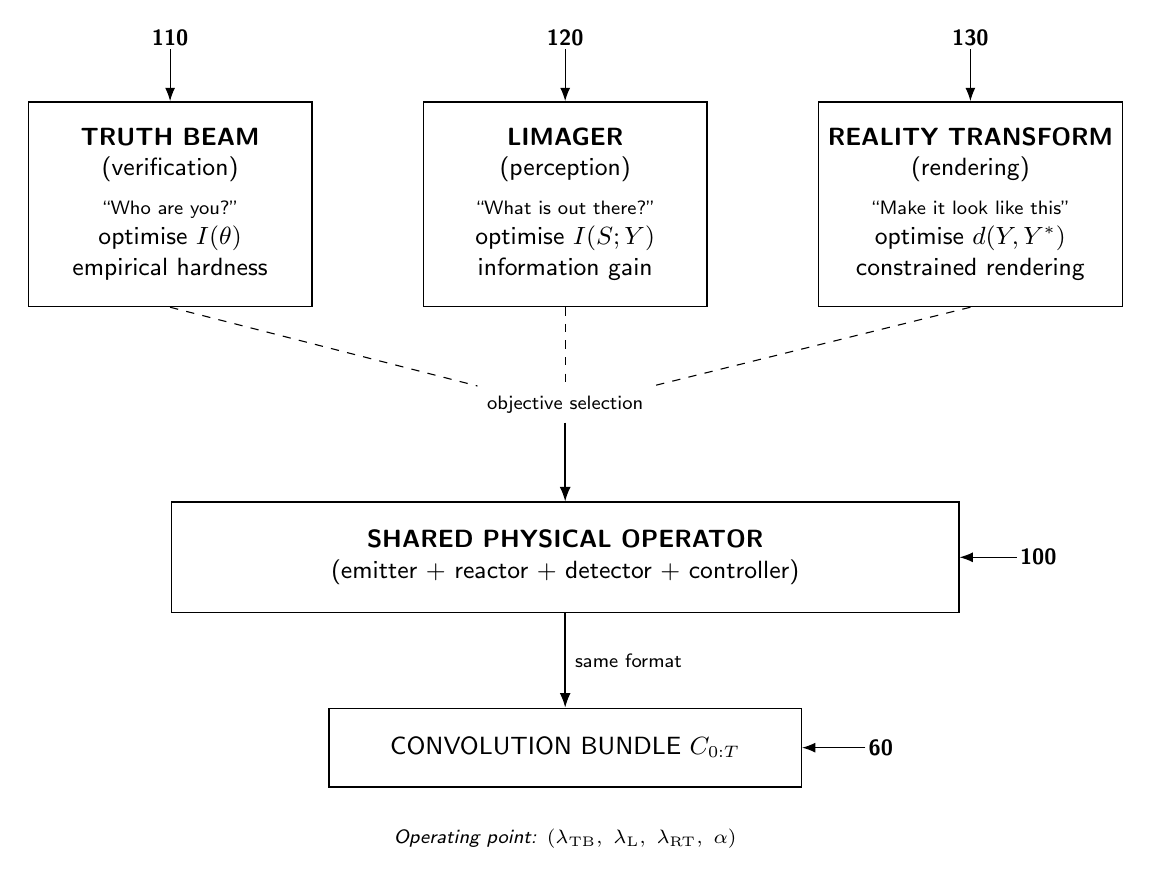
\begin{tikzpicture}[node distance=8mm]

% Three regime boxes, top row
\node[cbox-tall, minimum width=3.6cm, minimum height=2.6cm] (tb)
  {\textbf{TRUTH BEAM}\\(verification)\\[3pt]
   \scriptsize ``Who are you?''\\optimise $I(\theta)$\\empirical hardness};
\node[cbox-tall, right=14mm of tb, minimum width=3.6cm, minimum height=2.6cm] (li)
  {\textbf{LIMAGER}\\(perception)\\[3pt]
   \scriptsize ``What is out there?''\\optimise $I(S;Y)$\\information gain};
\node[cbox-tall, right=14mm of li, minimum width=3.6cm, minimum height=2.6cm] (rt)
  {\textbf{REALITY TRANSFORM}\\(rendering)\\[3pt]
   \scriptsize ``Make it look like this''\\optimise $d(Y,Y^{*})$\\constrained rendering};

% Objective selection (dashed convergence)
\node[font=\scriptsize, below=10mm of li] (objsel) {objective selection};
\draw[line width=0.4pt, dashed] (tb.south) -- (objsel.north west);
\draw[line width=0.4pt, dashed] (li.south) -- (objsel.north);
\draw[line width=0.4pt, dashed] (rt.south) -- (objsel.north east);

% Shared physical operator 100
\node[cbox-wide, below=10mm of objsel, minimum width=10cm, minimum height=1.4cm] (op)
  {\textbf{SHARED PHYSICAL OPERATOR}\\
   (emitter + reactor + detector + controller)};
\draw[flowarr] (objsel.south) -- (op.north);

% Convolution bundle 60
\node[cbox-wide, below=12mm of op, minimum width=6cm, minimum height=1.0cm] (bundle)
  {CONVOLUTION BUNDLE $C_{0:T}$};
\draw[flowarr] (op.south) -- node[right, font=\scriptsize] {same format} (bundle.north);

% Operating point note
\node[font=\scriptsize\itshape, below=4mm of bundle, text width=12cm, align=center] (opnote)
  {Operating point: $(\lambda_{\mathrm{TB}},\ \lambda_{\mathrm{L}},\ \lambda_{\mathrm{RT}},\ \alpha)$};

% Reference numerals
\node[refnum] at ($(tb.north)+(0,8mm)$) (n110) {\textbf{110}};
\draw[leader] (n110.south) -- (tb.north);
\node[refnum] at ($(li.north)+(0,8mm)$) (n120) {\textbf{120}};
\draw[leader] (n120.south) -- (li.north);
\node[refnum] at ($(rt.north)+(0,8mm)$) (n130) {\textbf{130}};
\draw[leader] (n130.south) -- (rt.north);
\node[refnum] at ($(op.east)+(10mm,0)$) (n100) {\textbf{100}};
\draw[leader] (n100.west) -- (op.east);
\node[refnum] at ($(bundle.east)+(10mm,0)$) (n60) {\textbf{60}};
\draw[leader] (n60.west) -- (bundle.east);

\end{tikzpicture}
\end{center}

\end{document}
